\section{Experiment}
\label{sec:experiment}
\subsection{Feature Engineering}
\label{sub:feature_engineering}



\begin{table}[htpb]
   \centering
   \caption{Average processing time.}
   \label{tab:timing}
   \begin{tabular}{|c|r|r|r|r|r|r|}
      \hline
      \multirow{2}{*}{Algorithms} & \multicolumn{2}{c|}{Feature extraction} &
      \multicolumn{4}{c|}{Training} \\ \cline{2-7}
                     & Raw   & Smooth & Raw     & Raw FFT  & Smooth   & Smooth FFT \\ \hline
      AdaBoost       & 15.71 & 14.94  & 2026.13 & 35766.15 & 13109.74 & 32991.03\\
      Elastic net    & 16.60 & 16.06  & 151.96  & 577.30   & 121.73   & 537.47\\
      Gradient boost & 12.55 & 12.52  & 8090.82 & 45908.08 & 9695.63  & 46406.90\\
      Lasso          & 16.23 & 16.14  & 145.09  & 507.52   & 139.83   & 567.07\\
      NNR            & 15.78 & 15.59  & 18.75   & 33.29    & 18.34    & 35.41\\
      Random forest  & 15.80 & 15.61  & 3139.64 & 9236.24  & 3207.93  & 9380.83\\
      \hline
   \end{tabular}
\end{table}

\subsection{Benchmark}
\label{sub:benchmark}

\begin{figure}[htpb]
   \centering
   \subfloat[Relative error]{
      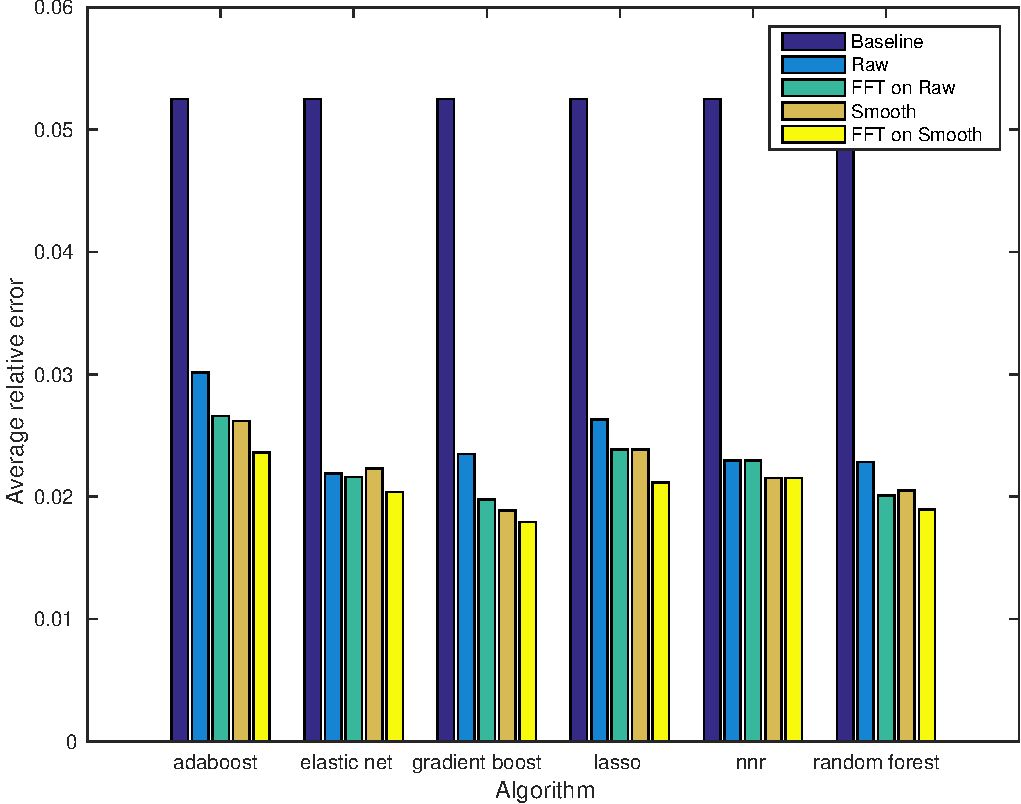
\includegraphics[width=0.45\linewidth]{figures/error_exp4_range50_rates8_pkts16.pdf}
   }
   \quad
   \subfloat[Standard derivation]{
      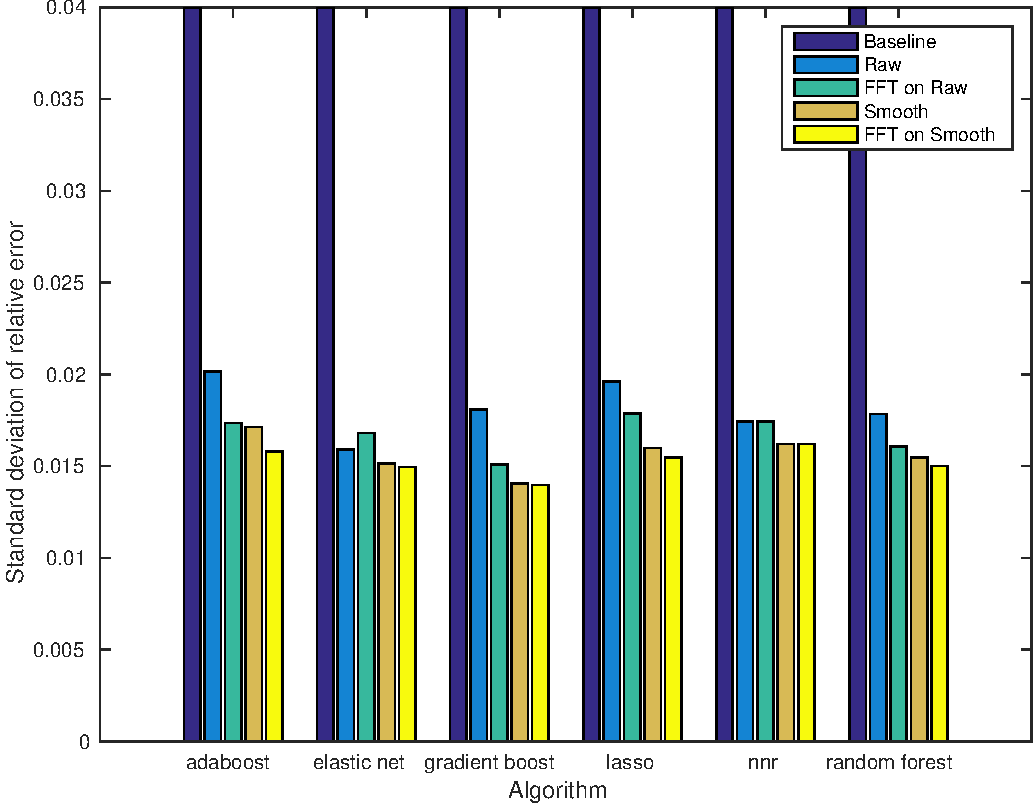
\includegraphics[width=0.45\linewidth]{figures/std_exp4_range50_rates8_pkts16.pdf}
   }
   \caption{Dataset: range 50, rates 8, packets 16}
   \label{fig:exp4}
\end{figure}

\begin{figure}[htpb]
   \centering
   \subfloat[Relative error]{
      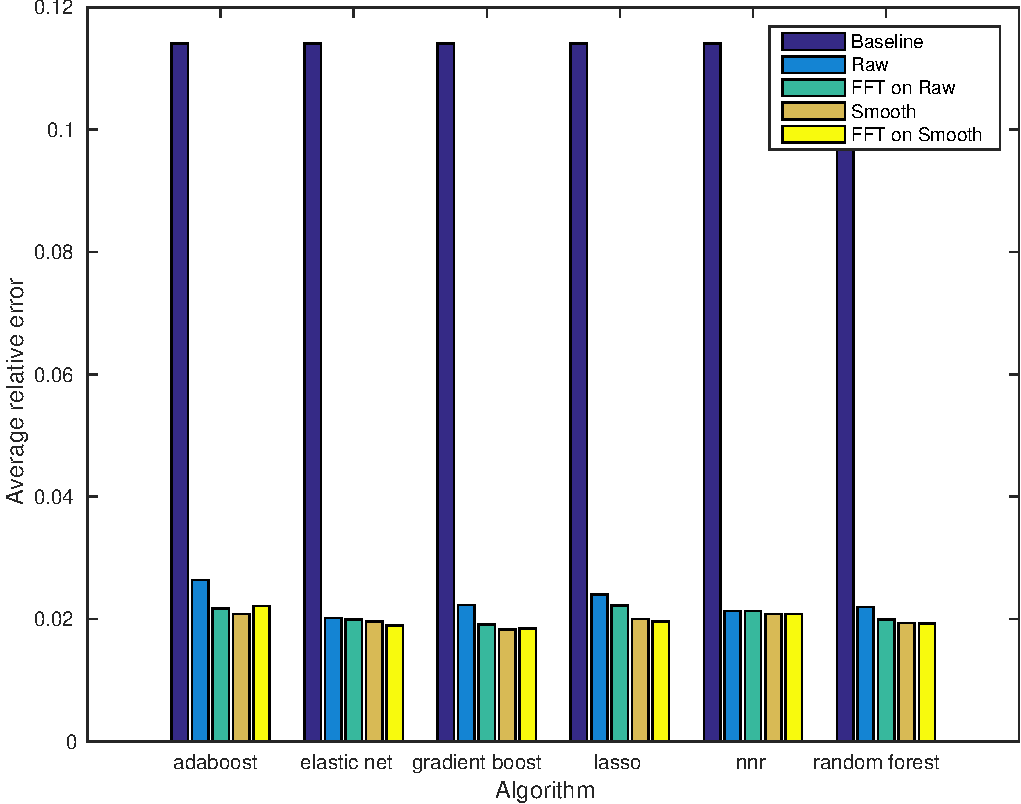
\includegraphics[width=0.45\linewidth]{figures/error_exp5_range50_rates2_pkts64.pdf}
   }
   \quad
   \subfloat[Standard derivation]{
      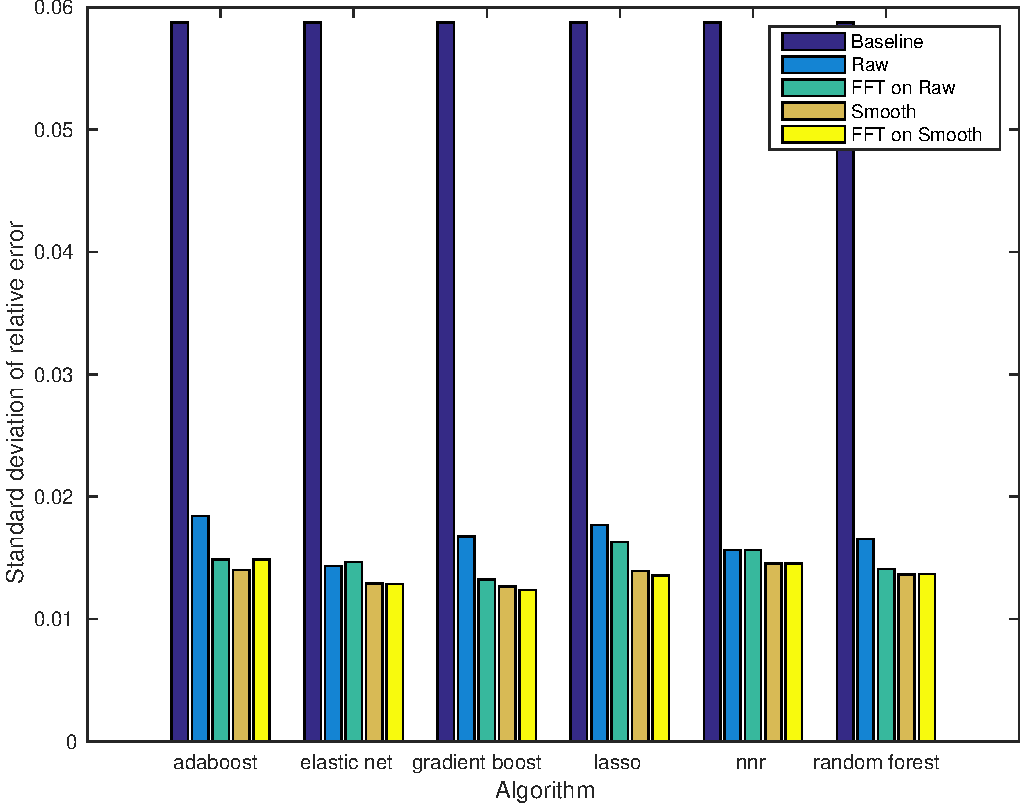
\includegraphics[width=0.45\linewidth]{figures/std_exp5_range50_rates2_pkts64.pdf}
   }
   \caption{Dataset: range 50, rates 2, packets 64}
   \label{fig:exp5}
\end{figure}

\begin{figure}[htpb]
   \centering
   \subfloat[Relative error]{
      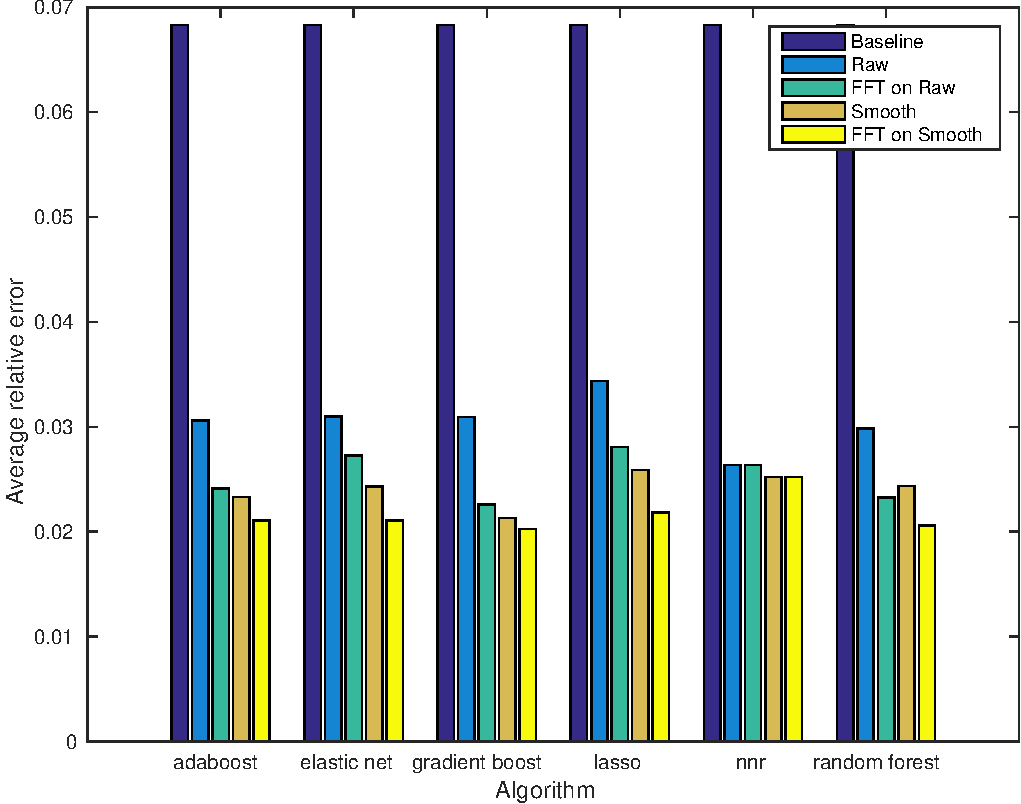
\includegraphics[width=0.45\linewidth]{figures/error_exp6_range50_rates3_pkts43.pdf}
   }
   \quad
   \subfloat[Standard derivation]{
      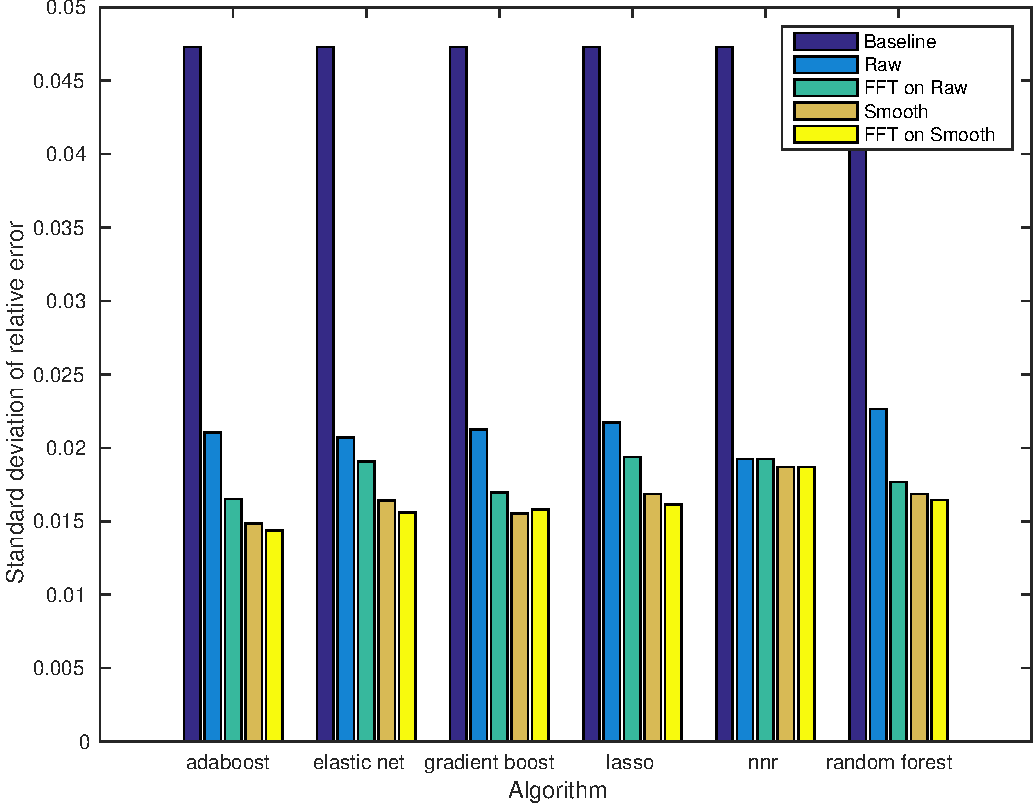
\includegraphics[width=0.45\linewidth]{figures/std_exp6_range50_rates3_pkts43.pdf}
   }
   \caption{Dataset: range 50, rates 3, packets 43}
   \label{fig:exp6}
\end{figure}

\begin{figure}[htpb]
   \centering
   \subfloat[Relative error]{
      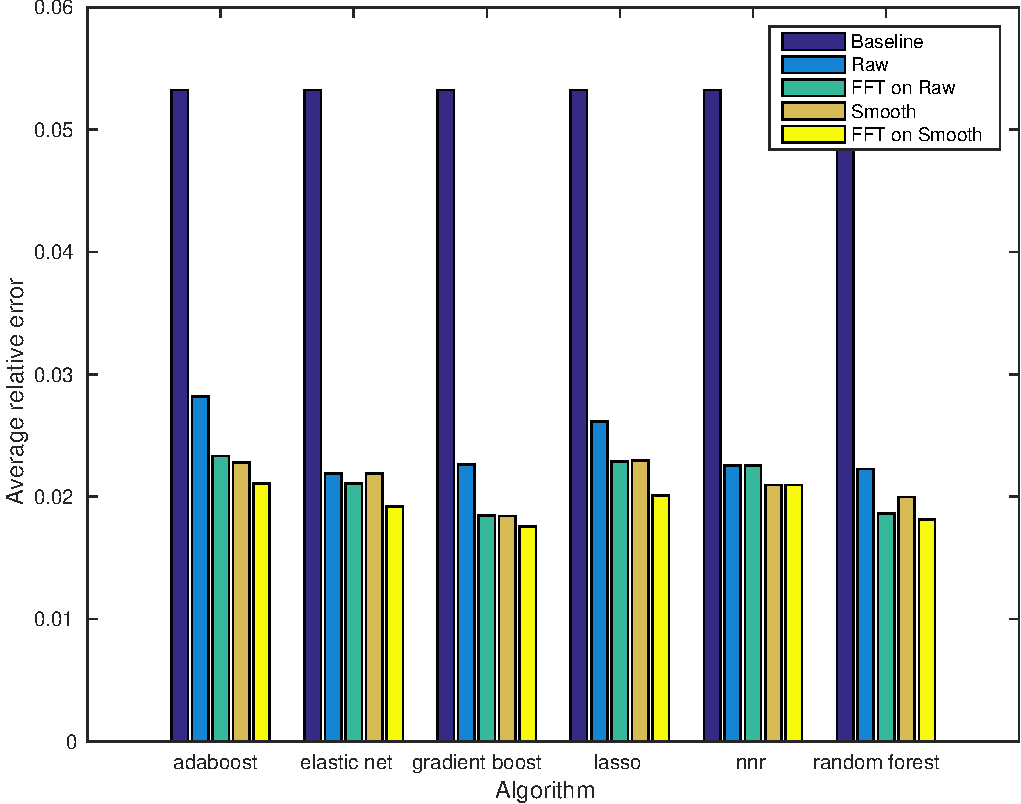
\includegraphics[width=0.45\linewidth]{figures/error_exp7_range50_rates6_pkts21.pdf}
   }
   \quad
   \subfloat[Standard derivation]{
      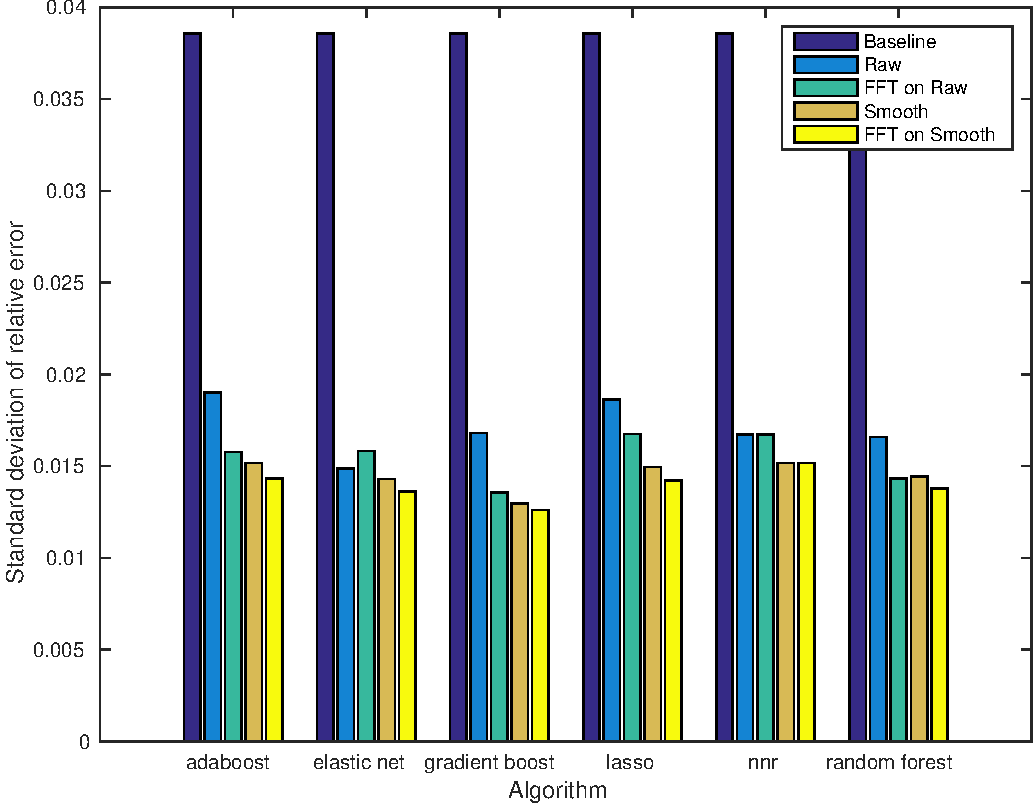
\includegraphics[width=0.45\linewidth]{figures/std_exp7_range50_rates6_pkts21.pdf}
   }
   \caption{Dataset: range 50, rates 6, packets 21}
   \label{fig:exp7}
\end{figure}

\begin{figure}[htpb]
   \centering
   \subfloat[Relative error]{
      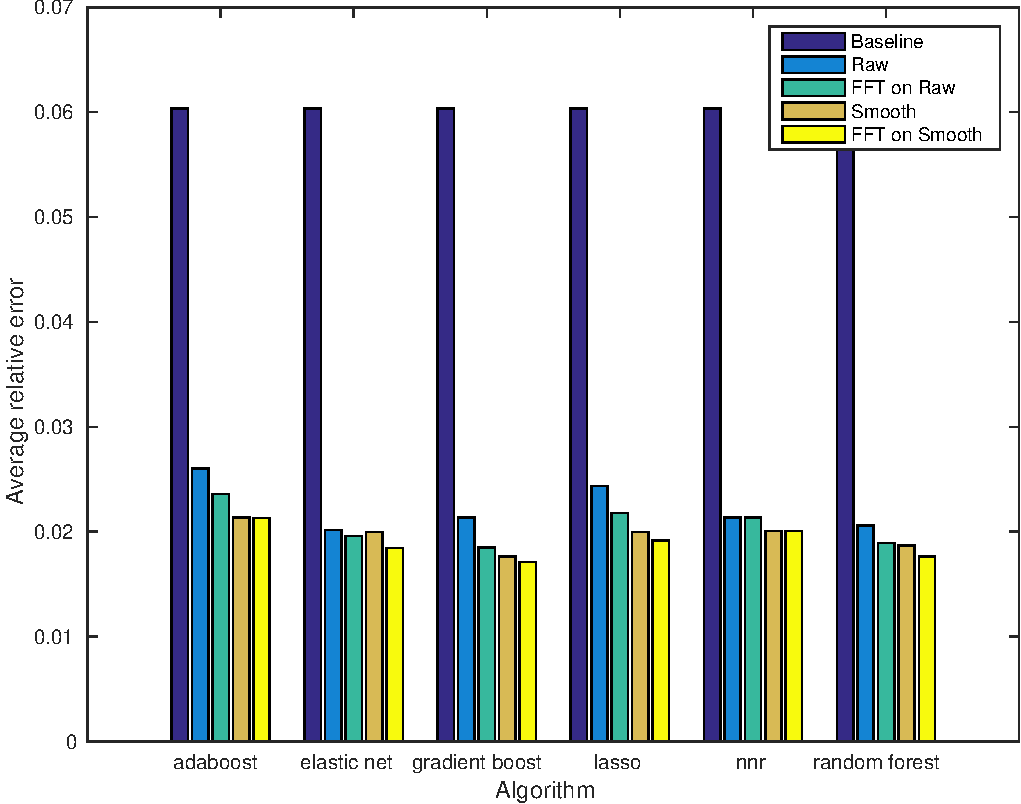
\includegraphics[width=0.45\linewidth]{figures/error_Nov9_range50_rates4_pkts32.pdf}
   }
   \quad
   \subfloat[Standard derivation]{
      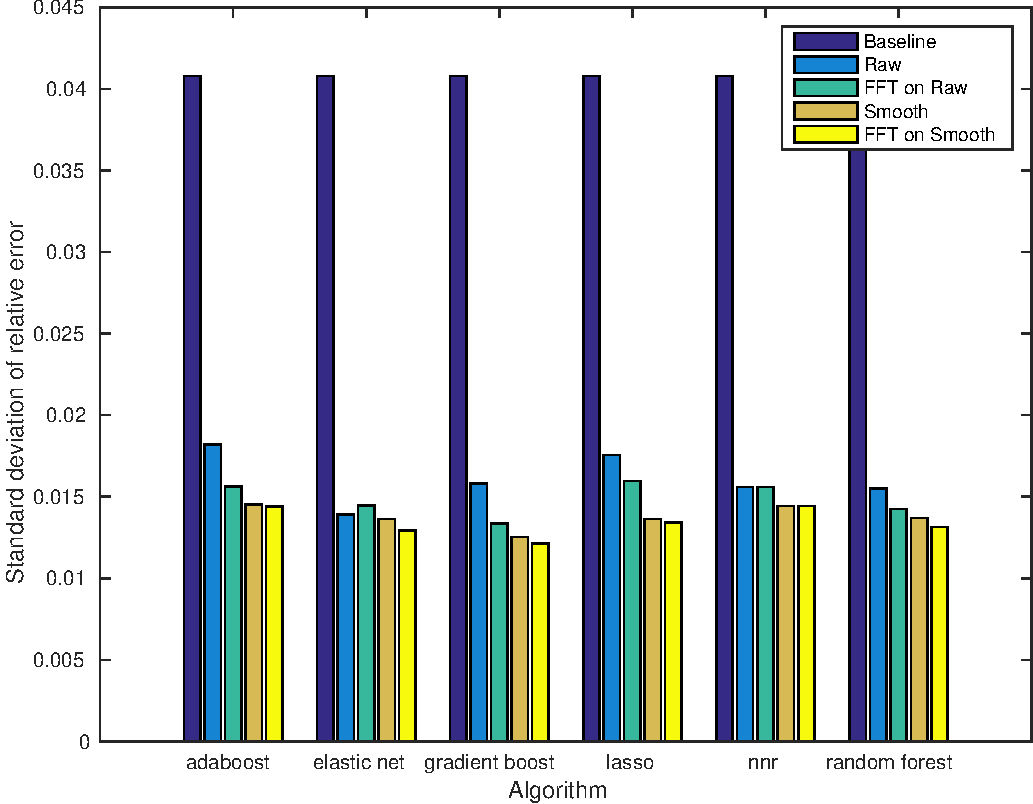
\includegraphics[width=0.45\linewidth]{figures/std_Nov9_range50_rates4_pkts32.pdf}
   }
   \caption{Dataset: range 50, rates 4, packets 32}
   \label{fig:nov9}
\end{figure}
